\chapter{Data Acquisition}
\label{chapt:DATA_ACQUISITION}
\section{Background}
\subsection{HTML and Xpath}

Internet webpages are written in HTML. When a webpage is accessed, the HTML code is sent to the user, and the browser processes and displays the webpage in a human-readable format. 

A scraping program must process the raw HTML file and access the useful information on the page in an automated fashion. Information is arranged in an HTML document in a tree-like structure (figure \ref{fig:HTMLTREE}). This example page would display as a table with three rows, each row containing `Table Data A/B/C'. This data is accessible programmatically using an `XPath'. 
\begin{figure}[H]
    \centering
    \textbf{HTML and XPaths}\par\medskip
    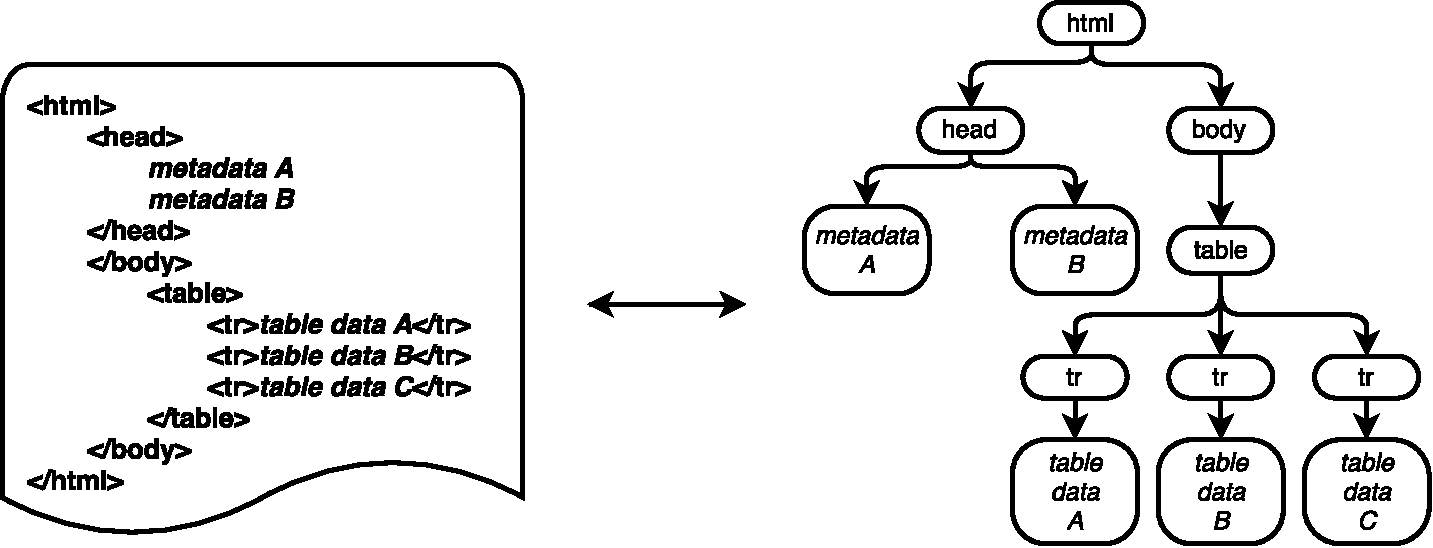
\includegraphics[width=\textwidth]{Data_Acquisition/html_tree.pdf}
    \caption[Tree representation of HTML Code]{Tree representation of HTML code. The html code here displays a table with three rows. The page has two pieces of meta-data associated with it, stored in the `head'.}
\label{fig:HTMLTREE}
\end{figure}
XPaths are simply paths through the tree to the desired information. In order the `scrape' the data in the table, the following XPath could be used:
\begin{center}
\texttt{//html/body/tr/*}
\end{center}
Scraping millions of webpages potentially requires millions of different XPaths. It is impractical to specify them manually, thus the challenge of large-scale scraping is how to identify and collect useful data on webages without manually specifying many XPaths.
\section{Collection Strategy}
The initial approach was to analyse the HTML tree to automatically recognise useful data generate XPaths\footnote{This approach is detailed in the appendix, \S\ref{sec:auto_xpaths}}. When this strategy proved unsuitable, a new method was required. Chemical information is usually disseminated as journal articles accompanied by a DOI. By programmatically collecting DOIs, (\S\ref{sec:DOI}) it was possible to build up a large database of chemical information (\S\ref{sec:SCRAPING_PROGRAM})
\subsection{DOIs : Document Object Identifiers}
\label{sec:DOI}
DOIs are computer-friendly labels for articles. DOIs are issued by a number of accredited bodies, with the majority issued by Crossref \cite{crossref-formation}. By pre-pending a DOI with the url stub \texttt{http://dx.doi.org/}, The IDF service redirects the request to the publisher's website to display the article the DOI refers to. The DOI structure is shown in figure \ref{fig:DOI}.
\begin{figure}[H]
    \centering
    \textbf{Anatomy of a DOI}\par\medskip
    \includegraphics[width=0.6\textwidth]{Data_Acquisition/DOI2.png}
    \caption[Anatomy of a DOI]{DOI structure. The structure consists of a numeric prefix (X and Y must be integers) and alphanumeric suffix (Z can be any Unicode-encoded character)} \label{fig:DOI}
\end{figure}
DOIs consist of a prefix and a suffix. The prefix is subdivided into the ‘Directory Indicator’ \footnote{The Directory indicator has always been integer ‘10’ for every DOI issued at time of writing.} separated from the ‘Registrant Code’, assigned by the issuing body\cite{doi_handbook1}. Registrant codes are a minimum of three integers, with further optional subdivisions separated by full stops. The suffix is provided by the registrant and can be any form of unicode-encoded text\cite{doi_handbook1}.

It was possible to write a `Regular Expression' pattern (REGEX) to automatically recognise DOIs within a body of text (figure \ref{fig:REGEX}). The flexibility of the registrant code specification means that DOIs cannot always be unambiguously identified in HTML. 
\begin{figure}[H]
    \centering
    \textbf{Pattern Matching Procedure for DOIs}\par\medskip
    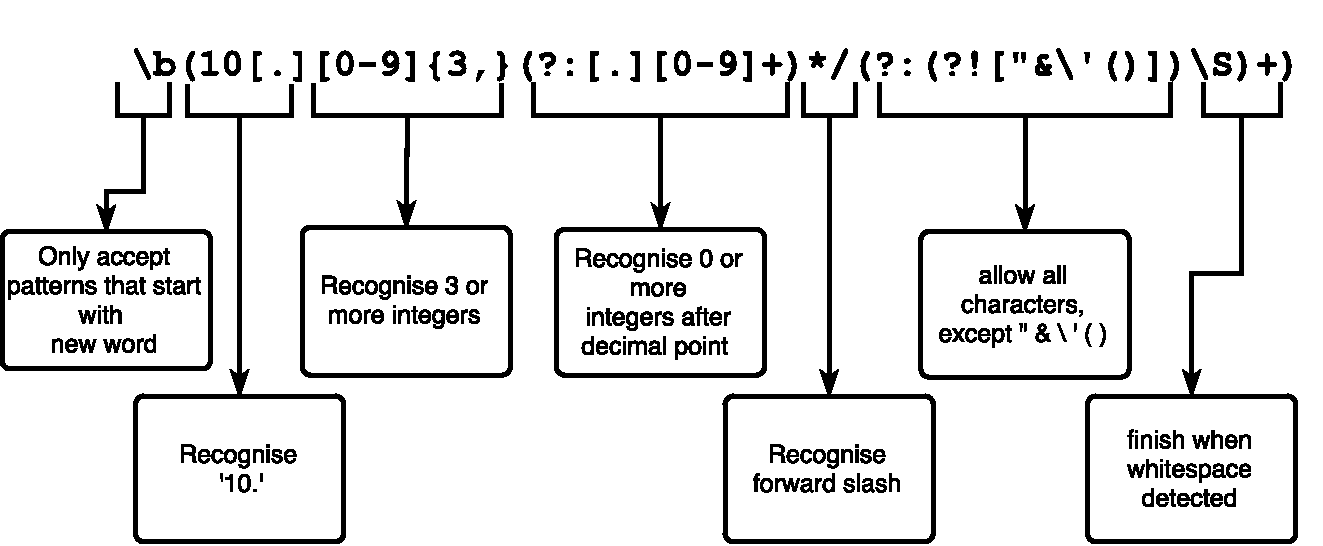
\includegraphics[width=\textwidth]{Data_Acquisition/Regex.pdf}
    \caption[Pattern Matching Procdure for DOIs]{Perl Syntax REGEX Code that can identify the vast majority of DOIs within free text} \label{fig:REGEX}
\end{figure}
The REGEX was able to identify 90.4\% of the DOIs on \url{http://www.ch.cam.ac.uk/publications}. 
\subsection{Scraping Program}
\label{sec:SCRAPING_PROGRAM}
The REGEX approach does not require XPaths in order to extract DOIs from a webpage. This facilitates large-scale scraping from many websites. Some meta-data\footnote{See Glossary for project-specific definition of meta-data} associated with a DOI can be accessed using an online API exposed by Crossref. The remaining meta-data can be accessed by following the \texttt{http://dx.doi.org/\{DOI\}} link to visit publishers' webpages.

With this methodology in place, a scraping program was written to collect DOIs from a list of webpages, collecting meta-data in a two stage process. The Crossref API provides article titles, journals, authors, publisher and publication date meta-data, but not article abstracts. These had to be collected by visiting publisher webpages, and collecting with hand written XPaths\footnote{Since there are comparatively few publisher websites, only 26 publisher XPaths were required for respectable capture coverage.}. The procedure is summarised in figure \ref{fig:Cherry}.
\begin{figure}[H]
    \centering
    \textbf{Scraping Procedure}\par\medskip
    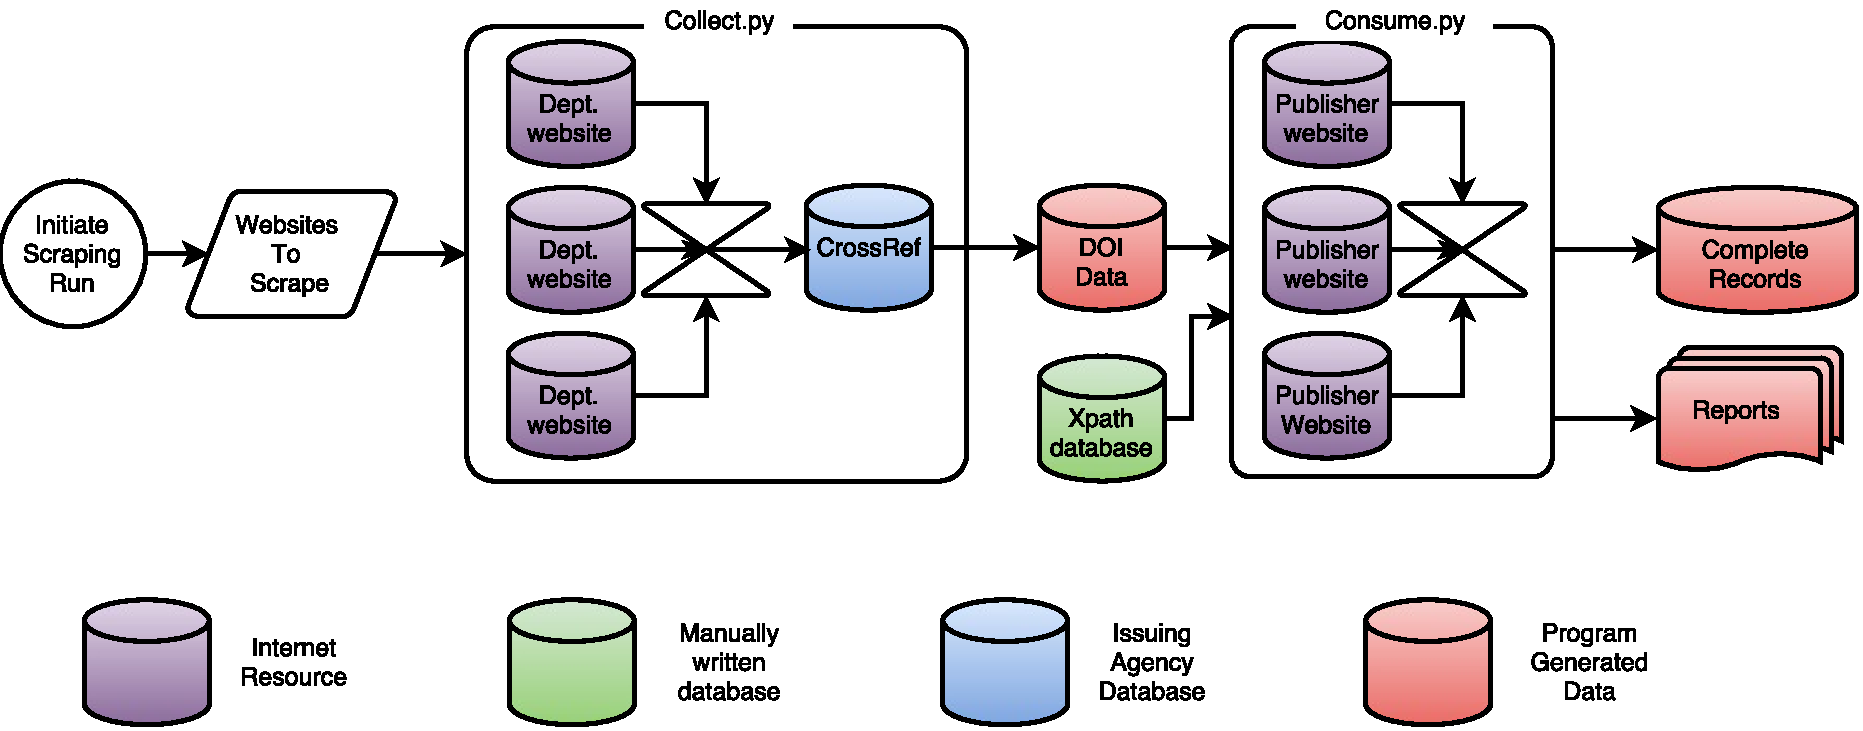
\includegraphics[width=\textwidth]{Data_Acquisition/Cherry2.pdf}
    \caption[Data Flow in Scraping Procedure]{The data flow of the scraping program. Websites from an inputted list of websites are visited and DOIs are extracted in the process described in  \S\ref{sec:DOI}. The Crossref API service is then used to verify the extracted DOIs, and collects available meta-data. The program then accesses publisher webpages and collects abstracts. The program also produces explanation of capture failures and some general statistics}
\label{fig:Cherry}
\end{figure}
The programmatic steps depicted in figure \ref{fig:Cherry} are:
\begin{sloppypar}
\begin{enumerate}
\itemsep-0.5em 
\item \texttt{Request the webpage from the inputted list}
\item \texttt{Process the html and extract DOIs}
\item \texttt{Using the Crossref Online API, verify the extracted DOIs exist}
\item \texttt{Crossref yields metadata:}
\begin{itemize}
\itemsep-0.5em 
\item \texttt{Title}
\item \texttt{Journal}
\item \texttt{Publisher}
\item \texttt{Authors}
\item \texttt{Publication Date}
\end{itemize}
\item \texttt{For each DOI,  follow \texttt{http://dx.doi.org/\{DOI\}} link}
\item \texttt{Use XPath to collect article abstracts}
\end{enumerate}
\end{sloppypar}
The program exports complete records as .json files, but also feeds to a MongoDB database. Once the program was written, a list of webpages to scrape was required. \S\ref{sec:UKSCRAPE} and \S\ref{sec:CROSSREFSCRAPE} describe how this was achieved.
\section{Collection Results}
\subsection{UK University Department scraping}
\label{sec:UKSCRAPE}
The program was first used to collect the data from the UK. The Goodman group's website hosts a list of UK chemistry departments \url{http://www-jmg.ch.cam.ac.uk/data/c2k/uk.html}. The list was manually checked and edited to give a list of 68 departments\footnote{Details can be found in the appendix, \S\ref{sec:data_acc_appendix}.}. The program was run using this list, the results of which are detailed in table \ref{tab:UKSCRAPERES}. The DOIs collected were stored in database $\Delta1$ and the complete results were stored in database $\Delta2$.
\begin{table}[H]
\caption{UK Scraping results}
\label{tab:UKSCRAPERES}
\begin{center}
\begin{tabular}{||l|l|l||}
\hline
Process & \# records & \% of maximum yield\\
\hline
Dois collected & 22442 & N/A\%\\
Dois found with metadata & 22397 & 99.8\%\\
Articles successfully resolved & 16363 & 72.9\%\\
Losses due to failed requests & 2753 & 12.3\%\\
Program errors & 133 & 0.6\%\\
Missing Publication Errors & 3148 & 14.0\% \\
\hline
\end{tabular}
\end{center}
\end{table}
Conversion losses were due to four components. 45 losses for non-existant DOIs, 2753 to request errors (404 : not-found errors or permission problems), 133 to the program errors and 3148 to missing publication XPaths. The 26 specified XPaths \footnote{Corresponding to 37 publishers.} were sufficient to convert 83.8\% of successful requests. This was deemed acceptable, as most major publishers had been covered\footnote{See appendix for list of covered publishers, \S\ref{sec:data_acc_appendix}.}, and the missing publishers each covered a small number of articles\footnote{It would take another 11 XPaths of the missing most popular publishers to increase the conversion rate from 83.8\% to 90\%.}
The efficiency is depicted in figure \ref{fig:UKSANK}.

\begin{figure}[H]
    \centering
    \textbf{Efficiency of UK Department Scraping}\par\medskip
    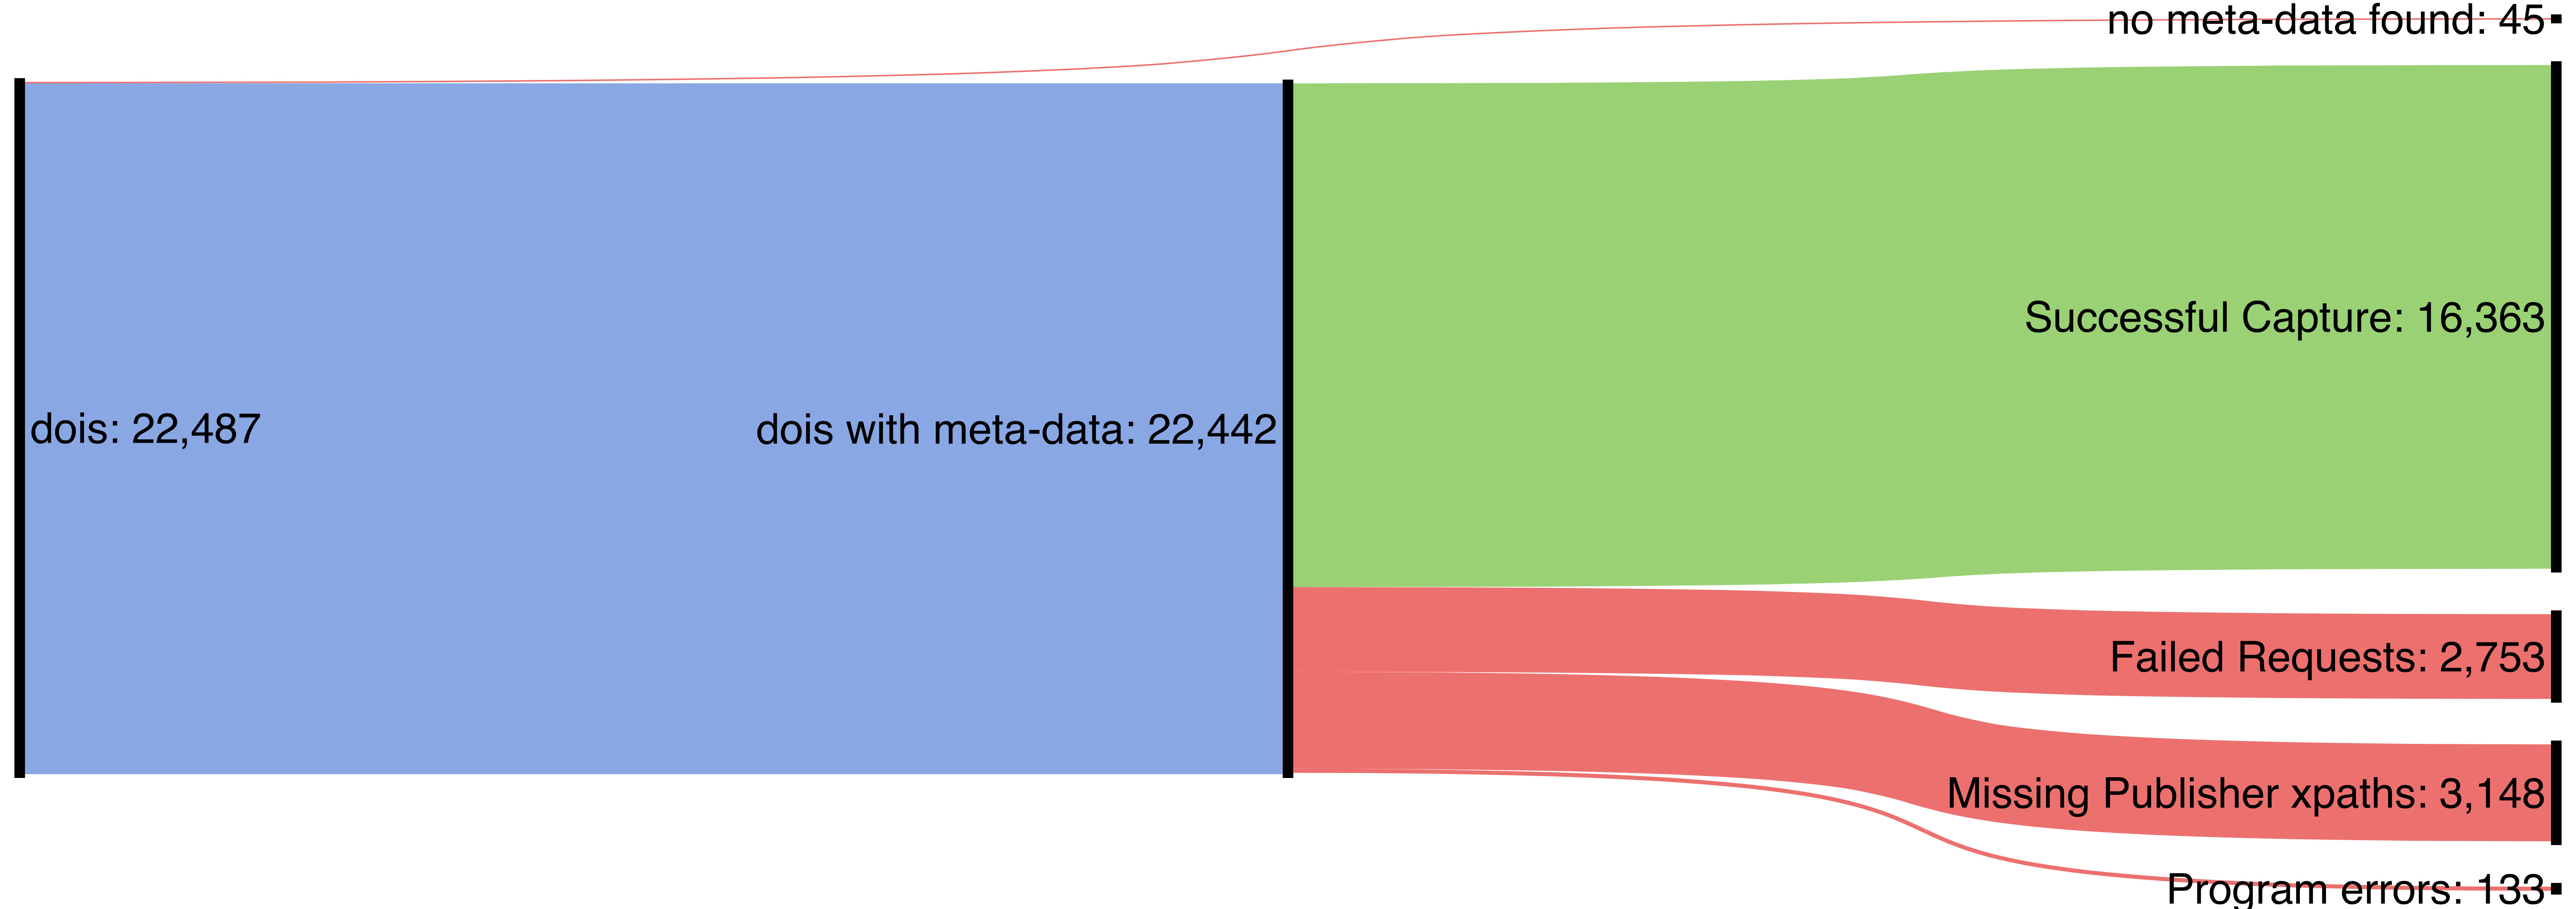
\includegraphics[width=\textwidth]{Data_Acquisition/uk_sankey.png}
    \caption[Efficiency of UK Department Scraping]{The loss processes are coloured red, successfully captured full records in green, and the maximum possible yield in blue.}
     \label{fig:UKSANK}
\end{figure}

Interestingly, 9467 out of 16363 successful collections were sourced from \url{http://www.ch.cam.ac.uk}. This could be because the department at Cambridge has an extensive website and  hosts the majority of its information under its own domain name, whereas other departments' data are hosted on central university domains. The program was instructed to only scrape webpages belonging to chemistry department domains, not university websites as a whole. It is noted that the Cambridge chemistry department may be overrepresented in $\Delta2$.

\subsection{Global Scale Scraping}
\label{sec:CROSSREFSCRAPE}
Much more data would be required to train a successful machine learning model. One approach would have been to expand to world-wide chemistry departments and other learn\`{e}d bodies. However, Crossref also exposes a search service that can be used to query its vast internal database. The program was set up to query the Crossref service for search terms `Chemistry', `Chemical', `Molecule' and `Molecular' for journal articles and journal titles. This suggested possible yields in the millions of articles. 

The program was instructed to scrape the search-result pages of these queries. Because the scraping job was large, it was programmed to `pause' before publisher abstract collection. The results up to this point were examined before setting off the second stage to collect abstracts.

At the intermediate point, the program had collected 1,267,495 records. This database was labelled $\Delta3$. Publisher distributions and potential server loads were then carefully considered and capture probabilities were predicted before the second half of the scraping routine was set off to run for three days\footnote{Some of this analysis is presented in \S\ref{sec:SCRAPEANALYSIS}.}.
\label{sec:CROSSREFSCRAPE}
\subsection{Problems with ACS and Taylor \& Francis}
\label{sec:banning1}
Most publishers track request volumes sent to their servers to discourage automatic downloading. Scraping constitutes fair use and complies to UK copyright law. Despite the university owning a full-access licence to these publishers' publications, the collected material was freely available without licence\cite{thelaw} \cite{contentminelegal}. During the scraping run, a bug in the randomisation of requests resulted in detection by ACS and Taylor \& Francis, which responded by banning the computer's IP address \footnote{Explored in detail in \S\ref{sec:banning2}}. The department librarians were able to restore access, and it was agreed that no further scraping would be performed.
\subsection{Analysis of collected data}
The yield of the global-scale scraping run was cut significantly by the ACS banning. A summary is tabulated in table \ref{tab:LARGESCRAPERES} and shown graphically in figure \ref{fig:LARGESANK}. The complete records were stored in database $\Delta4$.
\begin{table}[H]
\caption{Global Scraping Results}
\label{tab:LARGESCRAPERES}
\begin{center}
\begin{tabular}{||l|l|l||}
\hline
Process & \# records & \% of maximum yield\\
\hline
DOIS collected &  1267495 &N/A\\
DOIS collected with meta-data &  1267495 &100.0\%\\

\hline
Predicted maximum capture & 1071506 &  84.5\%\\
Predicted Capture without ACS & 581797 & 45.9\%\\
\hline
Articles successfully captured & 714370 & 56.4\%\\
Losses to failed requests (excluding ACS)& 53743 & 4.2\%\\
Losses to ACS banning & 303393 & 23.9\%\\
Missing Publications \& Program Errors & 195989 & 15.5\%\\
\hline
\end{tabular}
\end{center}
\end{table}
\begin{figure}[H]
    \centering
    \textbf{Efficiency of Global Scraping}\par\medskip
    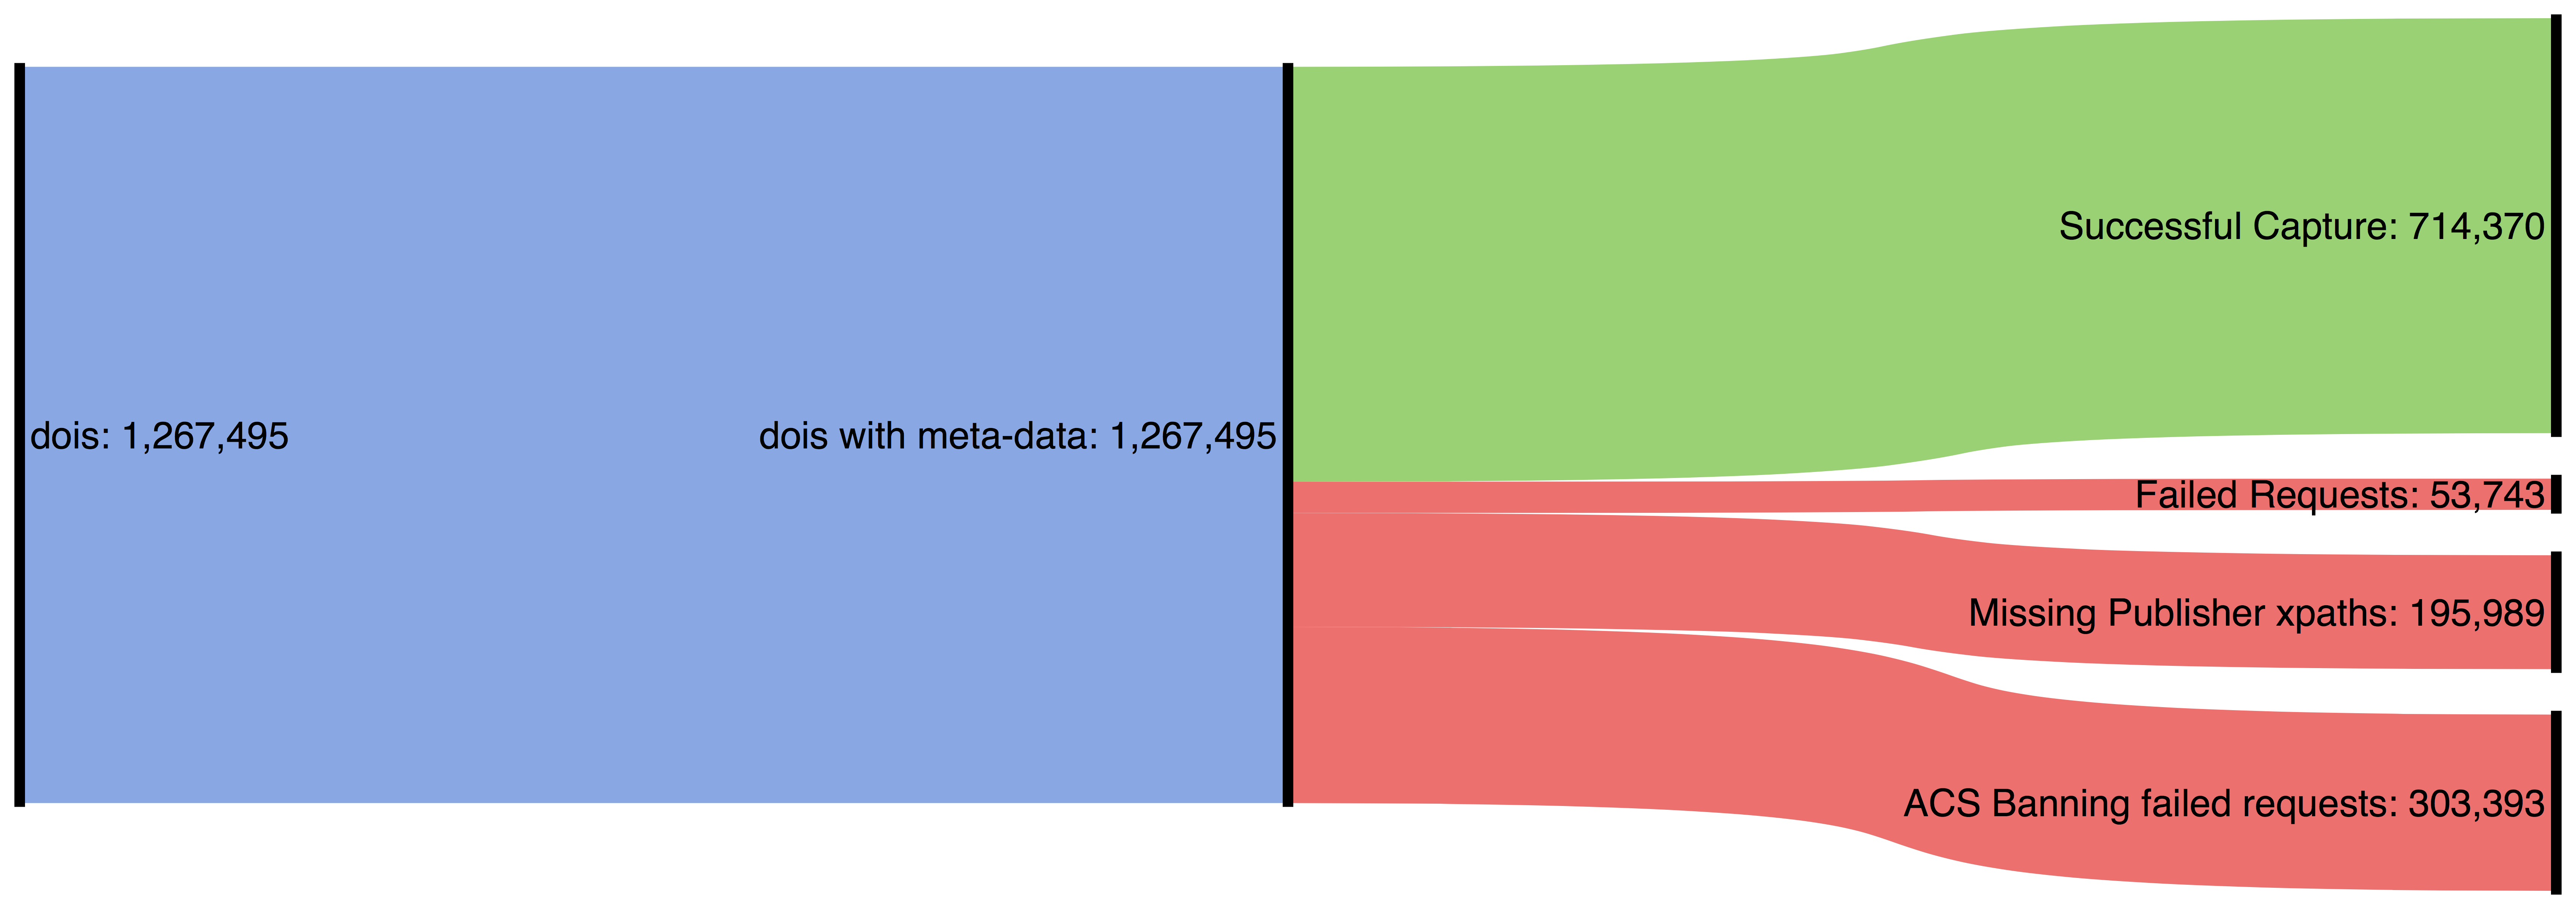
\includegraphics[width=\textwidth]{Data_Acquisition/large_sankey.png}
    \caption[Efficiency of Large Scale Scraping]{The loss processes are coloured red, successfully-captured full records in green, and the maximum possible yield in blue.}
     \label{fig:LARGESANK}
\end{figure}

The overall efficiency of the process is 56.4\%, but excluding lost ACS records, the program's efficiency was 74.0\%, similar to the efficiency of the UK scrape (\S\ref{sec:UKSCRAPE})\footnote{Also note that 100\% of DOIs were converted to DOIs with meta-data. This was because the format of the webpages scraped was consistent for every DOI collected.}.

The successful 714,370 records were merged with the UK results\footnote{The merged dataset was labelled $\Delta5$}. Records were rejected with short titles or abstracts, or if the majority of the title and abstract were not written in ascii characters\footnote{Likely to be addenda, informal articles, retractions etc, and removing removing majority Japanese and Chinese script.}. This was done to provide higher-quality data for algorithm training (see \S\ref{chapt:ALGORITHM}). This filtering resulted in a final training database of 464712 articles. This dataset was labelled $\Delta6$. The database formation process is summarised in figure \ref{fig:DATABASES} and table \ref{tab:DATABASES}.
\begin{figure}[H]
    \centering
    \textbf{Summary of Database Preparation}\par\medskip
    \includegraphics[scale=0.6]{Data_Acquisition/Databases2.pdf}
    \caption[Summary of Database Preparation]{Blue databases ($\Delta1$, $\Delta3$) represent data with DOIs and meta-data. Green databases ($\Delta2$, $\Delta4$ ) represent meta-data, DOIs and abstracts. The purple database ($\Delta5$) is the combined complete records, and the red database is the data deemed suitable for the training algorithm. Database Populations and losses are annotated.}
     \label{fig:DATABASES}
\end{figure}
\begin{table}[H]
\caption{Databases created in Data Acquisition Process}
\label{tab:DATABASES}
\begin{tabular}{||c|c|c|c||}
\hline 
Database &  Contents & \# Records\\
$\Delta1$ & Dois found on UK Chemistry Department websites & 22,397 \\
$\Delta2$ & Complete meta-data obtained from records in $\Delta1$ & 16,363 \\
$\Delta3$ & Dois found in global scraping using crossref API & 1,267,495  \\
$\Delta4$ & Complete meta-data obtained from records in $\Delta3$ & 714,370 \\
$\Delta5$ & Complete records obtained from combining $\Delta2$ and $\Delta4$ & 730,733 \\
$\Delta6$ & Records appropriate for training taken from $\Delta5$ & 464,712 \\
\hline
\end{tabular}
\end{table}

It was instructive to examine these databases and derive some simple statistical results, which is explored in \S\ref{sec:CORPUSOBSERVATIONS}.